The Auto Regressive Integrated Moving Average (ARIMA) model is a time series model where the ARIMA analyse time series with a class of stochastic processes \cite{EnergyPriceForecasting,ARIMA}. The model has been applied to forecast of commodity prices such as oil, gas and electricity \cite{ARIMA}. 

The success of the presented ARIMA model is dependent on the linear relationship of the underlying data generating process, whereas the Artificial Neural Network can handle non-linear relationships \cite{1}. The Artificial Neural Networks are simple but a very powerful tool when it comes to forecasting, provided that the training set contains enough data and that enough computational resources are available. 
In \cite{1} the Artificial Neural Network outperforms the ARIMA model in terms of both time consumption and accuracy of the predicted price as shown in ~\ref{fig:ArimaVSNN}. where the error percentage to the actual price is shown.
\begin{figure}[h!]
\centering
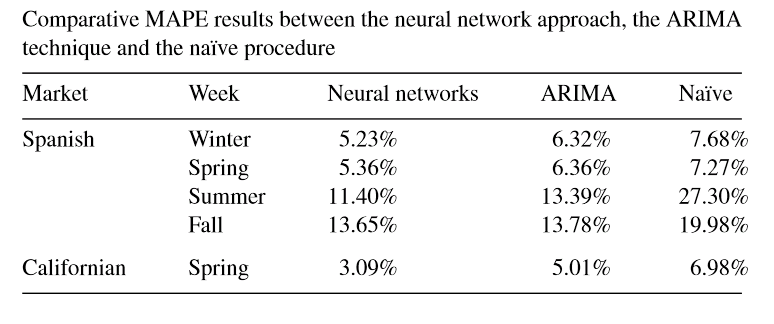
\includegraphics[width=0.8\linewidth,natwidth=898,natheight=587]{billeder/ARIMAvsNN.png}
\caption{Comparison between Neural Network and ARIMA in terms of error \cite{1}}
\label{fig:ArimaVSNN}
\end{figure}